\documentclass{article}

\usepackage[utf8]{inputenc}
\usepackage[T1]{fontenc}
\usepackage[british]{babel}
\usepackage{lmodern}
\usepackage{microtype}
\usepackage{siunitx}
\usepackage{circuitikz}
\usepackage{graphicx}
\usepackage{physics}
\usepackage[sorting=none, giveninits=true]{biblatex}
\usepackage[hidelinks]{hyperref}
\bibliography{pe3}

\title{PE3 proposal:\\ Measuring thermal noise in resistors}
\author{Luuk de Jong -- s2260018}
\date{April 2024}

\begin{document}
\maketitle
\begin{center}
  Group a \\
  Lecturer: Dr.ir. P.S.W.M. Logman 
\end{center}
\section{Introduction}
Thermal noise is present in all electronics, and limits the sensitivity of instruments.
While noise is often sought to be minimised, it may be of interest to measure and characterise it directly.
This research aims to directly measure thermal noise in resistors, study its dependence on resistance and temperature, and introduce a robust and reproducible device to easily do so.
\subsection{Theory}
Unlike ideal resistors, real resistors introduce noise in a signal, caused by thermal agitation of the electrons\cite{nyquist_thermal_1928}.
Thermal noise is a form of white noise, with the spectrum depending only on temperature and resistance\cite{wagenaar_physics_2023}, shown in \autoref{eq:noise-spectrum}.
\begin{equation}
  \label{eq:noise-spectrum}
  S_{\mathrm{V}}(f) = 4k_{\mathrm{B}}TR
\end{equation}
Given a bandwidth $\Delta f$, the noise power is
\begin{equation}
  \label{eq:noise-power}
  \sigma_{\mathrm{V}}^2 = 4k_{\mathrm{B}}TR\Delta f.
\end{equation}
\subsection{Research Question and Hypothesis}
The following question will be researched:
\begin{quote}
  What is the relation between thermal noise and the temperature and resistance of a resistor, as measured using a sensitive amplifier?
\end{quote}
The following subquestions will to this end be investigated:
\begin{itemize}
\item \textit{What is the gain $G(f)$ of the amplifier?}
  This will depend on the exact components chosen, but it is expected to of an order $10^3$, with a maximum around $\SI{2}{\kHz}$.
\item \textit{What is the background noise of the amplifier?}
  This will again depend on the specifics of the amplifier, as well as the environment, but it is expected to be of order $\SI{1}{\mV}$.
  % \item \textit{What is the input capacitance of the amplifier?}
  %   This again depends on the specifics of the sensor, but it expected to be of order
  %   \SI{1}{\pF}.
\item \textit{What is the noise power of a resistor with resistance $R$ and temperature $T$?}
  This is expected to follow \autoref{eq:noise-power}, where $\Delta f$ depends on the input capacitance of the system.
\end{itemize}
Hypothesis: the noise power obeys \autoref{eq:noise-power}.
\section{Methods}
\subsection{Setup}
% The setup and methods are based on those used by Thaned Pruttivarasin\cite{pruttivarasin_robust_2018}, who in turn based his work on Joe Geller's work\cite{geller_build_2007}.
The setup and methods are those used by Thaned Pruttivarasin\cite{pruttivarasin_robust_2018}, who in turn based his work on Joe Geller's work\cite{geller_build_2007}.
The amplifier uses two operational amplifiers and a \textsc{jfet}.
The system is powered by two \SI{9}{\V} batteries, as these produce less noise than a power supply.
The input and output are connected to grounded \textsc{bnc} connectors.
To shield the system from outside noise, it is enclosed in an aluminium box or paint can.
\autoref{fig:circuit} shows a diagram of the circuit.
Due to the high paracitic capacitance of breadboards, this system is best made on a circuit board.

\begin{figure}[h]
  \centering
  \resizebox{\linewidth}{!}{
    \begin{circuitikz}
      \node[njfet](jfet) at (0, 0) {};
      \draw (jfet.G) to[short] ++(-0.5, 0) node(R1i){}
        to[C=\SI{100}{\nF}] ++(-2, 0)
        node[bnc](input){input \textsc{bnc}};
      \draw (jfet.S) to[short] ++(0, -2) node[ground](gnd0){};
      \draw (input.shield) to[short] (input.shield |- gnd0)
        to[short] (gnd0);
      \draw (R1i.center) to[R=\SI{10}{\mega\ohm}] (R1i |- gnd0);
      \draw (jfet.D) to[R=\SI{1}{\kohm}] ++(0, 1.5)
        to[battery, label=\SI{9}{\V}] ++(0, 1) node[ground, rotate=180]{};
      \draw (jfet.D) to[C=\SI{1}{\uF}] ++(2, 0) node[op amp, anchor=-](oa1){};
      \draw (oa1.+) node[ground]{};
      \draw (oa1.-) to[short] ++(0, 1) coordinate(R3i)
        to[R=\SI{39}{\kohm}] (R3i -| oa1.out) coordinate(R3f)
        to[short] (oa1.out);
      \draw (R3i) to[short] ++(0, 1.5) coordinate(C3i)
        to[C=\SI{150}{\pF}] (C3i -| R3f)
        to[short] (R3f);
      \draw (oa1.out) to[R=\SI{1}{\kohm}] ++(2, 0) coordinate(R4f)
        to[C=\SI{1}{\nF}] ++(0, -2) node[ground]{};
      \draw (R4f) to[C=\SI{1}{\uF}] ++(2, 0)
        to[R=\SI{1}{\kohm}] ++(2, 0)
        node[op amp, anchor=-](oa2){};
      \draw (oa2.-) to[short] ++(0, 1) coordinate(R6i)
        to[R=\SI{39}{\kohm}] (R6i -| oa2.out) coordinate(R6f)
        to[short] (oa2.out);
      \draw (R6i) to[short] ++(0, 1.5) coordinate(C6i)
        to[C=\SI{150}{\pF}] (C6i -| R6f)
        to[short] (R6f);
      \draw (oa2.+) node[ground]{};
      \draw (oa2.out) to[R=\SI{390}{\ohm}] ++(2, 0) coordinate(R7f)
        to[short] ++(1, 0)
        node[bnc,
             rotate=180,
             label={[anchor=south]below:output \textsc{bnc}}](output){};
      \draw (R7f)
        to[C, l_=\SI{150}{\pF}] ++(0, -2) node[ground](ground4){};
      \draw (output.north) |- (ground4);
    \end{circuitikz}  
  }
  \caption{
    A circuit diagram of the amplifier.
    The \textsc{jfet} should have a low input capacitance, like the 
    Linear Integrated Systems LSK189.
    The opamps should have low noise, such as the Linear Technology LT1028.
    The opamps are powered by a \SI{9}{\V} battery.
  }
  \label{fig:circuit}
\end{figure}

The output will be connected to a Rigol DS1052E oscilloscope.
A Tabor 8020 or Siglent SDG830 function generator will be connected to the input when measuring the gain.
For measuring the thermal noise, a metal film resistor inside a resistor box will be connected to the input.
\subsection{Measuring}
\subsubsection{Gain}
To measure $G(f)$, a function generator is connected to the input, and the input and output voltages are measured using the oscilloscope.
The gain $G = V_{\text{out}} / V_{\text{in}}$ is measured over a range of frequencies from $\sim\SI{10}{\Hz}$ to $\sim\SI{100}{\kHz}$.
The oscilloscope data can be either read out using a computer, or the $V_{\mathrm{RMS}}$ can be calculated by the oscilloscope itself.
Each datapoint is measured multiple times, to reduce measurements error and estimate uncertainty.
\subsubsection{Background noise}
By shorting the input and measuring the output, $V_{\mathrm{RMS}}$ for the background noise can be determined, to be later subtracted from the measurements.
\subsubsection{Thermal noise}
To measure the thermal noise, a resistor box is connected to the input, and $V_{\mathrm{RMS}}$ is measured using the oscilloscope.
As before, multiple measurements are conducted per data point.
This process is repeated for a variety of resistors.
\subsection{Analysis}
\subsubsection{Gain}
Using the obtained points of $V_{\text{in}}(f)$ and corresponding $V_{\text{out}}(f)$, the gain $G(f) = V_{\text{out}}(f) / V_{\text{in}}(f)$ can be calculated, as well as the standard deviation.
To use the gain to later calculate the real noise power from the measured output, $G$ is interpolated using SciPy.
\subsubsection{Background noise}
The obtained $V_{\mathrm{RMS}}$ of the background noise can later be used to correct the measured thermal noise.
By measuring the background noise multiple times, an uncertainty can be calculated.
\subsubsection{Thermal noise}
Having obtained $V_{\mathrm{RMS}}$ for a variety of resistors the thermal noise can be obtained by quadratically subtracting the  background noise, because they are uncorrelated noise:
\begin{equation}
  \label{eq:background-subtracted}
  V^2_{\text{RMS, thermal}} = V^2_{\text{RMS, measured}} - V^2_{\text{RMS, background}}
\end{equation}
The amplifier is not ideal: it has an input capacitance and does not amplify evenly over its bandwidth, so \autoref{eq:noise-power} cannot be used.
Instead, the noise power is given \autoref{eq:real-noise-power}
\begin{equation}
  \label{eq:real-noise-power}
  V_{\mathrm{RMS}}^2 = 4k_{\mathrm{B}}TRG_{\mathrm{eff}}
\end{equation}
Here, $G_{\mathrm{eff}}$ is the effective gain, integrated over the bandwidth, taking into account the input capacitance of the amplifier and the resistance.
\begin{equation}
  \label{eq:effective-gain}
  G_{\mathrm{eff}} = \int_0^{\infty}\frac{G(f)^2}{1 + (2\pi fCR)^2}\dd{f}
\end{equation}
\autoref{fig:input-capacitance} show how the resistor attached to the input acts as an RC-filter, leading to \autoref{eq:effective-gain}
\begin{figure}[h]
  \centering
  \begin{circuitikz}
    \draw (0, 1) to[R=$R$, o-] ++(2, 0) to[short, -o] ++(2, 0);
    \draw (0, 0) to[short, o-o] ++(4, 0);
    \draw (2, 1) to[C=$C$] ++(0, -1);
    \node at (0, 0.5) {$V_{\text{noise}}$};
    \node at (4, 0.5) {$V_{\text{input}}$};
  \end{circuitikz}
  \caption{
    Th\'evenin equivalent of the test resistor attached to the input.
    $V_{\text{noise}}$ is the thermal noise, $R$ is the resistance of the resistor, and $C$ is the input capacitance of the system.
    The input acts as an RC-filter.
  }
  \label{fig:input-capacitance}
\end{figure}

The value for $C$ can be obtained by fitting the data using SciPy.
By using $k_{\mathrm{B}}$ as a fit parameter instead of a known constant, it too can be obtained from the measurements, providing both a way to determine $k_{\mathrm{B}}$ and a method to validate the results.
\section{Task Risk Analysis}
No significant risks are expected, as the system is powered using \SI{9}{\V} batteries, and the amplifier is not expected to be able to deliver a lot of current.
\begin{center}
  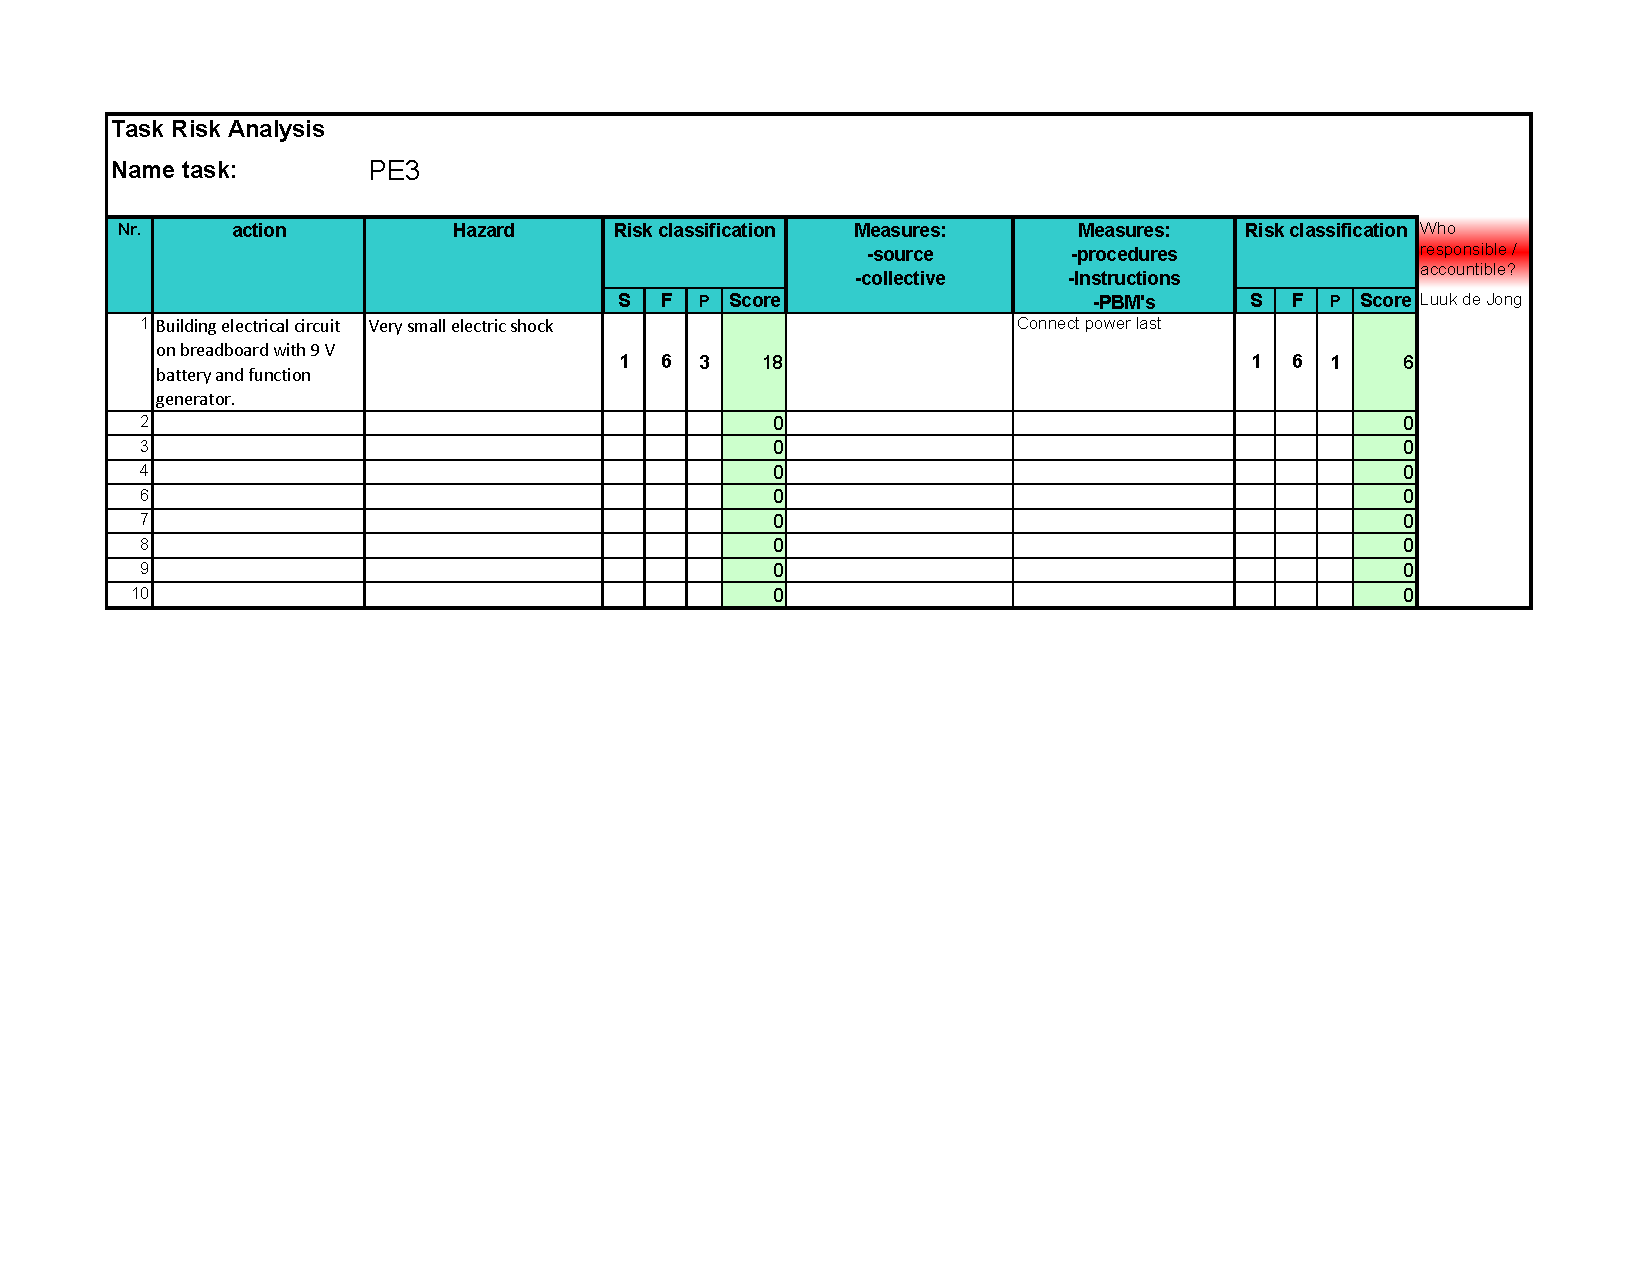
\includegraphics[width=\linewidth, trim={17mm, 112mm, 20mm, 19mm}, clip]{tra.pdf}
\end{center}
\printbibliography{}
\end{document}
